\section{Resultados}

\subsection{Aprendizaje supervisado}

Se puede apreciar que el accuracy para todos los modelos fue superior al 80\%. Por un lado es esperable altos valores del desempeño puesto que la etiqueta del diagnostico, que es la variable objetivo, esta construida a partir de un calculo con algunas de las variables independientes, es decir, los enunciados que corresponden al diagnostico. Por otra parte, lo realmente interesante es observar la distribución de la importancia de las variables que se utilizan para predecir la clase, así como que enunciados que no pertenecen al diagnostico y otro tipo de variables, terminan siendo importantes para el modelo.


Los resultados obtenidos por el grid search para modelo entrenado con los datos de la condición de estrés, se pueden apreciar en el cuadro \ref{table:modelo_estres} y la  importancia de las 20 variables mas importantes de dicho modelo en la figura \ref{variables_estress}.

\begin{table}[ht]
\centering
\caption{Métricas para el modelo de estrés}
\begin{tabular}{lllr}
\toprule
n\_estimators & max\_depth & criterion &  accuracy \\
\midrule
500 & 10 & entropy & 0.827264 \\
\bottomrule
\end{tabular}
\label{table:modelo_estres}
\end{table}%

\begin{figure}[h]
\caption{Importancia relativa de los atributos para el modelo de estrés}
\centering
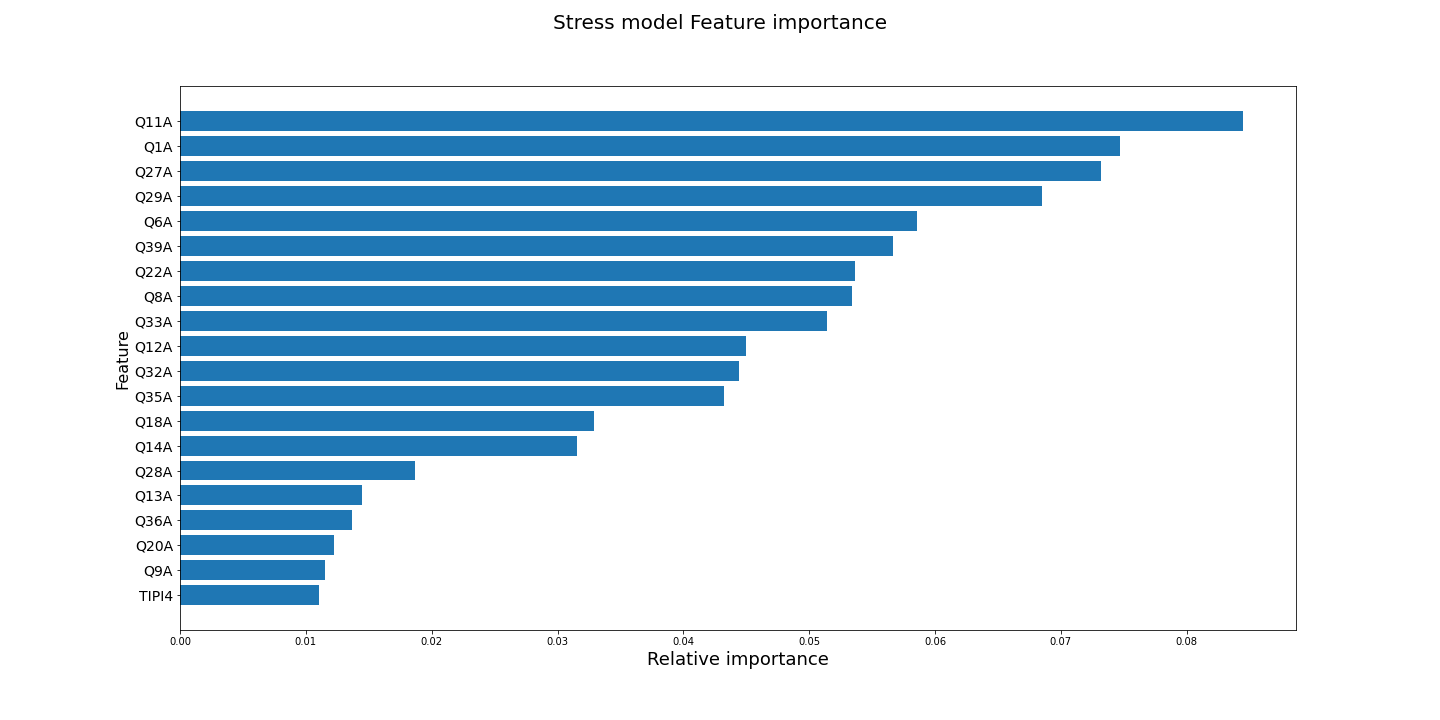
\includegraphics[width=\textwidth,height=\textheight,keepaspectratio]{Media/Pictures/Stress model Feature importance.png} 
\label{variables_estress}
\end{figure}



 \medbreak

Las variables que principalmente salen a las vista son aquellas que son utilizadas para el calculo del diagnostico, sin embargo, se puede apreciar que esta importancia no es constante para todas las preguntas que constituyen el test y que por el contrario, hay una diferencia significativa en la importancia que el modelo otorga a determinadas preguntas

 \medbreak

Hay un enunciado cuya importancia resalta que es la numero 11: "Me percibo molestándome con facilidad". Luego los enunciados 1, 27 y 29 tienen también un a importancia significativa y su valor es semejante; los enunciados son "Me percibo molestándome por cosas triviales'', "Me he encontrado siendo muy irritable" y ''Encuentro difícil calmarme después de que algo me ha molestado". Todos estos enunciados corresponden a la categoría de estrés y se aprecia como tienen en común la facilidad y frecuencia con la que el paciente suele molestarse.

 \medbreak
 
 Por otro lado, hay algunos enunciados que no corresponden a la categoría de estrés y que también son considerados importantes por el modelo, estos son 28, 36, 20 y 9 que pertenecen a la categoría de ansiedad y cuyos enunciados son "Me he sentido cerca al pánico", "Me he sentido aterrorizado", "Me he sentido asustado sin ninguna razón" y " Me he encontrado en situaciones que me hacen sentir tan ansioso que me he sentido casi aliviado cuando terminaron". Estos enunciados tienen en común el tema de la sensación de miedo sentido por el paciente. Además, también esta el enunciado 13 que corresponde a la categoría de depresión: "Me he sentido triste y deprimido". Finalmente, se aprecia que el enunciado 4 del TIPI también se considera importante para el modelo, cuyo enunciado es ''Ansioso, molesto fácilmente", lo cual va en concordancia con los enunciados encontrados mas importantes para el modelo.
 

 \medbreak
 
 Para la condición de ansiedad, los resultados del grid search se encuentran en el cuadro \ref{table:modelo_ansiedad} y la importancia delas 20 variables mas importantes esta en la figura \ref{variables_ansiedad} 
 

\begin{table}[ht]
\centering
\caption{Métricas para el modelo de Ansiedad}
\begin{tabular}{lllr}
\toprule
n\_estimators & max\_depth & criterion &  accuracy \\
\midrule
1000 & 10 & gini & 0.817404 \\
\bottomrule
\end{tabular}
\label{table:modelo_ansiedad}
\end{table}%

\begin{figure}[h]
\caption{Importancia relativa de los atributos para el modelo de Ansiedad}
\centering
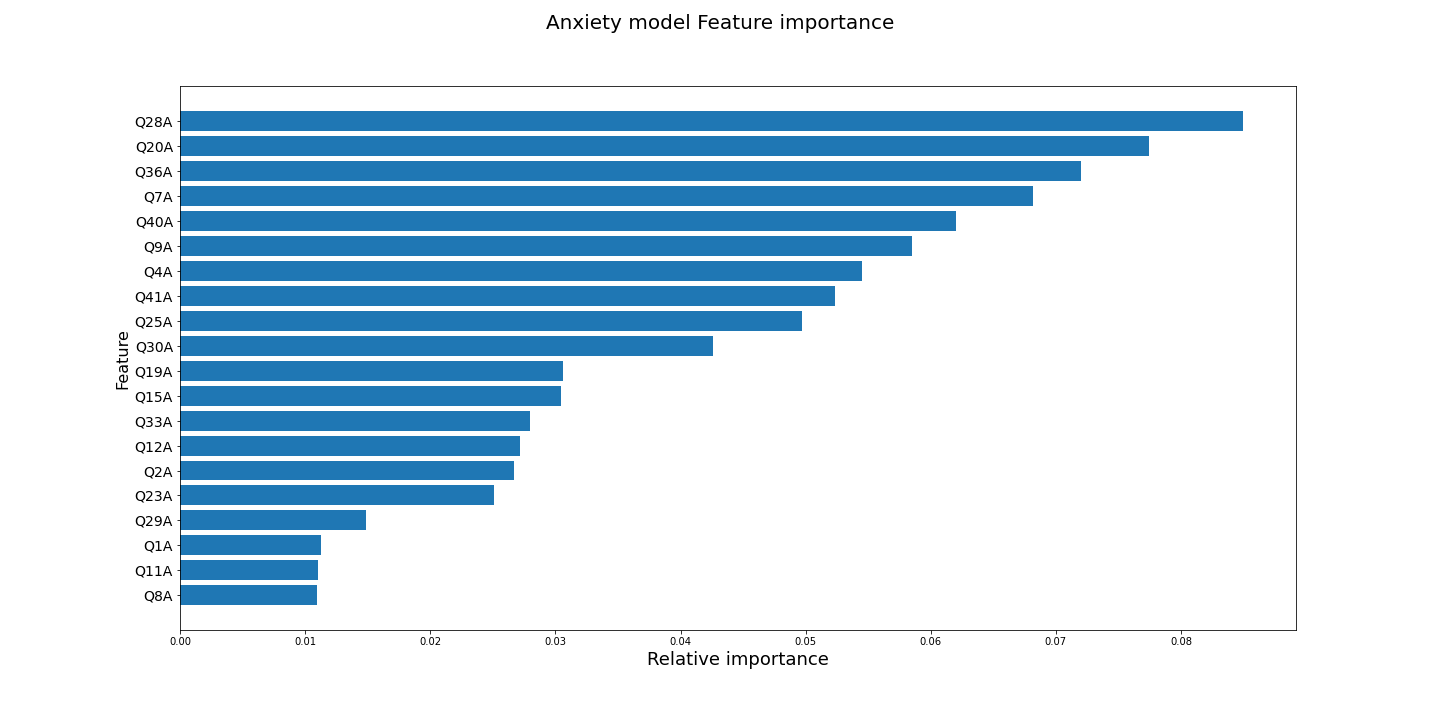
\includegraphics[width=\textwidth,height=\textheight,keepaspectratio]{Media/Pictures/Anxiety model Feature importance.png} 
\label{variables_ansiedad}
\end{figure}

Para este modelo, resalta que los principales enunciados son el 28, el 20, el 36 y el 7, que enuncian "Me he sentido cerca al pánico", "Me he sentido asustado sin ninguna razón", "Me he sentido aterrorizado" y "He tenido sensación de temblor". Resulta interesante que 3 de estos cuatro enunciados, es decir el 28, el 20 y el 36 también resultaron importantes para el modelo de estrés.

 \medbreak
 
Se puede apreciar que hay un quiebre en la importancia de las variables a partir del enunciado 19. Aquí encontramos mezclados enunciados que corresponden a la ansiedad y algunos que corresponden al estrés. Los de el estrés son  33, 12,  29, 1, 8 que enuncian "Me he sentido en un estado de tensión nerviosa", "He sentido que he usado mucha energía", ''Encuentro difícil calmarme después de que algo me ha molestado'', "Me percibo molestándome por cosas triviales'' y ''Encuentro difícil relajarme".Es de resaltar que las variable 29 y la 1 fueron de las mas importantes para el modelo de estrés, lo cual junto con las variables previamente mencionadas que también aparecen en el modelo de estrés, demuestra la alta correlación entre ambos observada en los datos.
 
Por otro lado, los enunciados que corresponden a ansiedad y que se encuentran luego de este quiebre de importancia son 19, 15, 2, 23 que enuncian ''Transpiro considerablemente  en la ausencia de altas temperaturas o ejercicio fisico'', ''He tenido sensación de desvanecimiento'', ''He sido consciente de la sequedad en mi boca'' y ''He tenido dificultad tragando'' respectivamente. Esto daría a entender que a la hora de diagnosticar esta condición, estos enunciados son igualmente importantes que los enunciados de estrés previamente mencionados.

 \medbreak

 Finalmente, para la condición de depresión, los resultados del grid search se encuentran en el cuadro \ref{table:modelo_depresion} y la importancia delas 20 variables mas importantes esta en la figura \ref{variables_depresion} 
 


\begin{table}[ht]
\centering
\caption{Métricas para el modelo de Depresión}
\begin{tabular}{lllr}
\toprule
n\_estimators & max\_depth & criterion &  accuracy \\
\midrule
1000 & 10 & gini & 0.878471 \\
\bottomrule
\end{tabular}
\label{table:modelo_depresion}
\end{table}%

\begin{figure}[h]
\caption{Importancia relativa de los atributos para el modelo de Depresión}
\centering
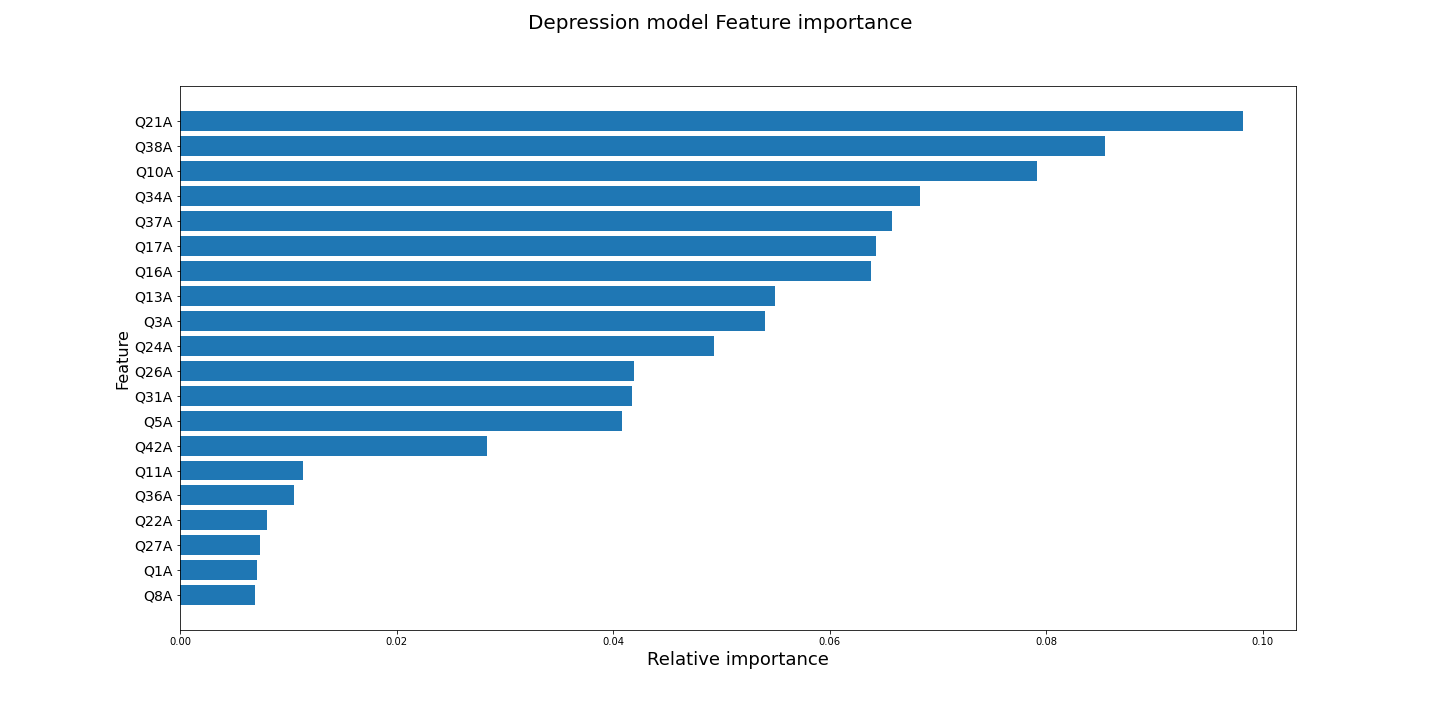
\includegraphics[width=\textwidth,height=\textheight,keepaspectratio]{Media/Pictures/Depression model Feature importance.png} 
\label{variables_depresion}
\end{figure}

Para el caso de la condición de depresión, resulta evidente que el enunciado mas importantes es el numero 21, que enuncia ''He sentido que la vida no vale la pena''. Luego los siguientes dos enunciados mas importantes son los numero 38 y 10 que enuncian ''He sentido que la vida no tiene sentido'', ''He sentido que no tengo nada a lo que aspirar''. Es interesante ver como estos tres enunciados denotan un desanimo general respecto a la vida.

 \medbreak

Por otro lado, dentro de estas 20 enunciados mas importantes se encuentran al final varios que tienen que ver con la condición de ansiedad; estos son los enunciados 11, 22, 27, 1 y  8 que enuncian "Me percibo molestándome con facilidad",  ''Encuentro difícil calmarme'',  , "Me he encontrado siendo muy irritable", "Me percibo molestándome por cosas triviales'' y  ''Encuentro difícil relajarme" respectivamente. De estos 4 enunciados, tres aparecen como los mas importantes del modelo de estrés, y estos son los enunciados 11, 1 y 27. A su vez el enunciado 1 apareció también como importante para el modelo de ansiedad. Esto muestra la alta correlación que tienen la depresión y el estrés, así como el hecho de que molestarse por cosas pequeñas se encuentra como importante en las tres condiciones.

 \medbreak

Finalmente, el enunciado numero 36 que corresponde a los enunciados de ansiedad también apareció dentro de los mas importantes y su enunciado es "Me he sentido aterrorizado", lo cual habla de la relación entre el miedo y la depresión.

 \subsection{Aprendizaje no supervisado}
 
 En la figura \ref{elbow_analysis} se encuentran los resultados de la implementación del método del codo en donde se puede apreciar el valor de la función de costo para los distintos números de clusters

\begin{figure}[h]
\caption{Costo total para diferente numero de Clusters}
\centering
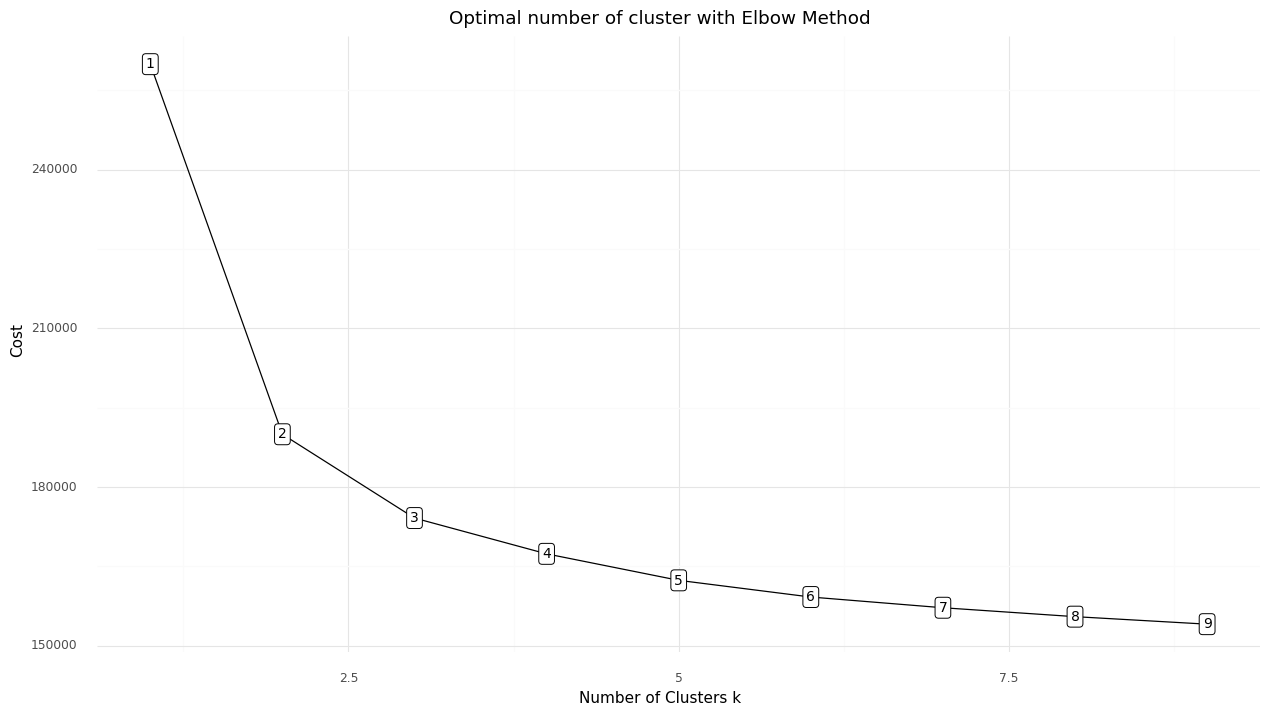
\includegraphics[width=\textwidth,height=\textheight,keepaspectratio]{Media/Pictures/elbow_analysis.png} 
\label{elbow_analysis}
\end{figure}

Se puede evidenciar un quiebre significativo de la pendiente a partir del numero 4 como cantidad de clusters, por lo que se elige esta cantidad.

\medbreak

Una vez entrenado el modelo y asignado un numero de cluster para cada caso, se procede calcular un perfil medio de los atributos demográficos para cada cluster cuyos resultados se encuentran en la figura \ref{perfiles_clusters}


\begin{table}[ht]
\centering
\caption{Perfil medio dentro de cada cluster}
\resizebox{\textwidth}{!}{\begin{tabular}{lrrrrrrrrrrrrrrrrrrr}
\toprule
{} &  education &  urban &  gender &  religion &  orientation &  race &  married &  TIPI1 &  TIPI2 &  TIPI3 &  TIPI4 &  TIPI5 &  TIPI6 &  TIPI7 &  TIPI8 &  TIPI9 &  TIPI10 &    age &  familysize \\
Cluster &            &        &         &           &              &       &          &        &        &        &        &        &        &        &        &        &         &        &             \\
\midrule
1       &  2.0 &  2.0 &  2.0 &  10.0 &  1.0 &  10.0 &  1.0 &  3.39 &  4.66 &  4.35 &  6.30 &  4.40 &  5.27 &  5.22 &  4.87 &  2.55 &  4.00 &  21.20 &  3.48 \\
2       &  2.0 &  2.0 &  2.0 &  10.0 &  1.0 &  10.0 &  1.0 &  3.25 &  4.23 &  4.38 &  5.39 &  4.71 &  5.18 &  5.12 &  4.53 &  3.18 &  3.84 &  23.22 &  3.29 \\
3       &  3.0 &  2.0 &  2.0 &  10.0 &  1.0 &  10.0 &  1.0 &  4.33 &  3.68 &  5.23 &  3.75 &  5.45 &  4.36 &  5.36 &  3.65 &  4.95 &  3.45 &  25.97 &  3.64 \\
4       &  3.0 &  2.0 &  2.0 &  10.0 &  1.0 &  10.0 &  1.0 &  3.99 &  4.28 &  4.86 &  5.47 &  5.04 &  4.73 &  5.36 &  4.23 &  3.65 &  3.71 &  22.83 &  3.53 \\
\bottomrule
\end{tabular}}
\end{table}%

Haciendo un paralelo con los perfiles encontrados previamente, se puede observar que el nivel educativo es mayor para los clusters 3 y 4. Así mismo la edad es mayor para el cluster 3 y menor para el cluster 1.  En cuanto al TIPI, los enunciados 1, 3, 5, y 9 tienden a ser mayores para el cluster 3 y menores para el cluster 1 y 4 siendo menores para los clusters 1 y 2; y los enunciados 2, 4, 6 y 8 son mayores para los clusters 1 y 2 y menores en los clusters 3 y 4. Esto invitaría a pensar que se esperan diagnósticos de severidad mayores principalmente en el cluster 1 y luego en el 2, encontrando las menores severidades en el cluster 3 y luego en el cluster 4


\medbreak
 
En la figura \ref{matriz_cluster_diagnosticos} se puede apreciar para cada cluster, cual fue la condición mas común para cada una de las condiciones. Se evidencia que el cluster 3 presenta principalmente diagnósticos normales, el 4 condiciones moderadas, el 2 una mezcla de distintos desde moderado a extremadamente severo y el cluster 1 son principalmente diagnósticos extremadamente severos. Esto es congruente con la información contenida en los perfiles demográficos.
 
 \begin{table}[ht]
\centering
\caption{Frecuencia máxima de diagnósticos por condición y cluster}
\begin{tabular}{lrrr}
\toprule
{} &  stress diagnosis & anxiety diagnosis & depression diagnosis \\
Cluster &                   &                   &                      \\
\midrule
1       &  Extremely severe &  Extremely severe &  Extremely severe \\
2       &  Moderate &  Severe &  Extremely severe \\
3       &  Normal &  Normal &  Normal \\
4       &  Moderate &  Moderate &  Moderate \\
\bottomrule
\end{tabular}
\label{matriz_cluster_diagnosticos}
\end{table}%
 
En el cuadro \ref{matriz_estres} se aprecia que la mayor cantidad de diagnósticos para el cluster 1 son severo y extremadamente severo, para el cluster 2 son moderado y severo y en menor medida leve y normal, para el cluster 3 son normal y leve y para el cluster 4 mayormente moderado, seguido de leve y severo y en menor medida normal. 

 
\begin{table}[ht]
\centering
\caption{Matriz de confusión para estrés}
\begin{tabular}{lrrrr}
\toprule
Clusters &     1 &     2 &     3 &     4 \\
Stress\_Diagnosis &       &       &       &       \\
\midrule
Normal           &  3 &  907 &  9743 &  1143 \\
Mild             &  9 &  1114 &  1090 &  2708 \\
Moderate         &  402 &  3442 &  212 &  4671 \\
Severe           &  3745 &  2717 &  6 &  2102 \\
Extremely severe &  5214 &  249 &  0 &  282 \\
\bottomrule
\end{tabular}
\label{matriz_estres}
\end{table}%

En el cuadro \ref{metricas_matriz_estres} se aprecian los valores de los índices de Van Dogen y y Rand ajustado, cuyos valores son 0.54 y 0.37 respectivamente, lo cual indica que aun cuando hay cierta afinidad entre los clusters creados y los diagnósticos para esta condición, estos no terminan de ser asignados de una manera completamente coincidente, en parte por que el numero de clusters es diferente al numero de condiciones y además hay cierta aleatoriedad en las asignaciones.


\begin{table}[ht]
\centering
\caption{Métricas de los clusters de estrés}
\begin{tabular}{rr}
\toprule
 Van Dongen Criterion &  Adjusted Rand Score \\
\midrule
0.54 & 0.37 \\
\bottomrule
\end{tabular}
\label{metricas_matriz_estres}
\end{table}%


 
 En las figuras \ref{clusters_estres}, \ref{clusters_ansiedad} y \ref{clusters_depresion} se muestran la comparación entre los clusters constituidos a la izquierda y el diagnostico de cada condición a la derecha, en una representación de dos dimensiones a través de la implementación de FAMD, en donde se puede apreciar la inercia, es decir, cuanta varianza es capaz de capturar, en cada eje. 

\medbreak

 
La figura \ref{clusters_estres} muestra como el eje x esta capturando la severidad de la condición de estrés, pues mientras los datos se ubican mas a la derecha, la severidad aumenta en la imagen de la derecha. En ese sentido, se aprecia que las condición normal esta claramente a la izquierda y la condición extremadamente severo bastante a la derecha, quedando así  un solapamiento entre las condiciones severa, moderada y media, estando la condición moderada en el centro. Por otro lado, la imagen de la izquierda nos muestra que los miembros del cluster 3 se ubican a la izquierda mientras que los miembros del cluster 1 se ubican a la derecha, quedando así los miembros del cluster 24 en la mitad con un poco de solapamiento entre ellos, estando el 4 a la izquierda y el 2 a la derecha. Esto es permite apreciar de una manera gráfica, cuan semejante es la distribución de las asignaciones previamente discutidas en el cuadro \ref{matriz_estres}


\begin{figure}[h]
\caption{Análisis de clusters para el diagnostico de estrés}
\centering
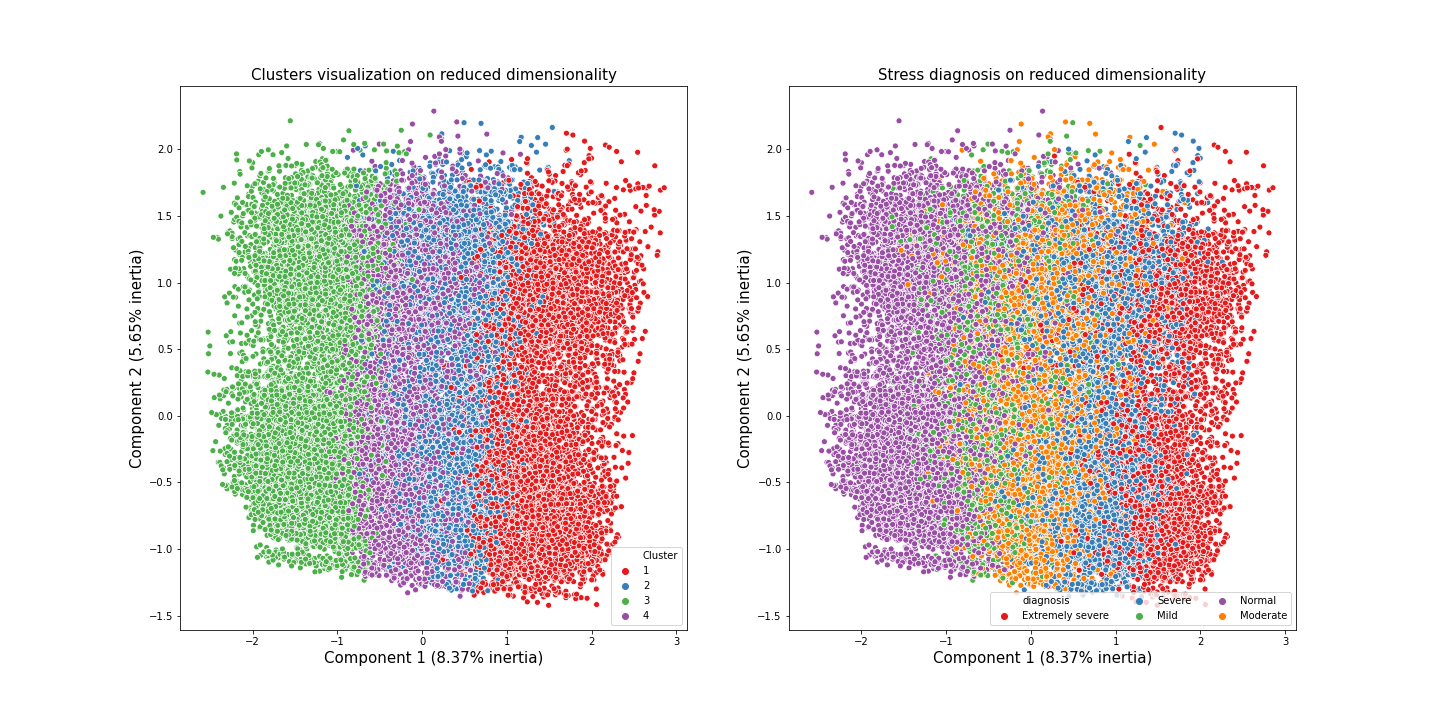
\includegraphics[width=\textwidth,height=\textheight,keepaspectratio]{Media/Pictures/stress_clusters.png} 
\label{clusters_estres}
\end{figure}

En el cuadro \ref{matriz_ansiedad} vemos como al cluster 1 son asignados principalmente casos con diagnostico extremadamente severo y en menor medida severo; el cluster dos tiene en proporcione similares diagnósticos moderados, severo y extremadamente severo, para luego tener mas presencia de de diagnostico normal que leve. El cluster 3 presenta principalmente diagnósticos normales y en una menor medida, diagnósticos leve, moderado y finalmente para el cluster 4 se presenten principalmente diagnósticos moderado y severo. Cabe resaltar la semejanza a las asignaciones que se dan para la condición de ansiedad con respecto a la condición de estrés, principalmente para los clusters 1 y  3 que presentan en su mayoría condiciones extremadamente severa y normales respectivamente, existiendo variaciones mas pronunciadas en los clusters 4 y 4 que tienen las condiciones intermedias. Esta semejanza puede verse así mismo en el cuadro \ref{metricas_matriz_ansiedad} ya que se tienen valores similares a los de la condición de estrés.

\begin{table}[ht]
\centering
\caption{Matriz de confusión para ansiedad}
\begin{tabular}{lrrrr}
\toprule
Clusters &     1 &     2 &     3 &     4 \\
Anxiety\_Diagnosis &       &       &       &       \\
\midrule
Normal            &  0 &  1031 &  7928 &  766 \\
Mild              &  0 &  549 &  1380 &  834 \\
Moderate          &  10 &  2216 &  1519 &  3302 \\
Severe            &  228 &  2561 &  213 &  3109 \\
Extremely severe  &  9135 &  2072 &  11 &  2895 \\
\bottomrule
\end{tabular}
\label{matriz_ansiedad} 
\end{table}%


\begin{table}[ht]
\centering
\caption{Métricas de los clusters de ansiedad}
\begin{tabular}{rr}
\toprule
 Van Dongen Criterion &  Adjusted Rand Score \\
\midrule
0.58 & 0.34 \\
\bottomrule
\end{tabular}
\label{metricas_matriz_ansiedad}
\end{table}%

En la figura \ref{clusters_ansiedad} puede verse que al igual que para la condición de estrés, para ansiedad el eje x esta capturando la severidad de la condición estando mas a la derecha condiciones mas severas. En ese sentido, si se compara con los clusters encontrados, se observa también que el cluster 3 al estar mas a la izquierda coincide con casos cuyos diagnósticos son menos severos, teniendo en el otro extremo al cluster 1, tal con mayor presencia de severidad en los diagnósticos. Se aprecia así mismo que los casos de ansiedad severa están mas dispersos hacia el centro superponiendo se con mas frecuencia a casos de diagnósticos severa y moderada, lo cual tendría que ver con el hecho de que para esta condición hay muchos mas casos con este diagnostico. Esto también tendría que ver con observar casos con diagnósticos de severidad extrema presentes hacia el centro de la gráfica, que corresponden a los clusters 2 y 4. Por otro lado, es también interesante el apreciar como los diagnósticos moderado y severa presentan una gran dispersión a lo lardo de la figura, lo cual coincide con su presencia en distintos clusters como lo muestra la matriz de confusión.


\begin{figure}[h]
\caption{Análisis de clusters para el diagnostico de ansiedad}
\centering
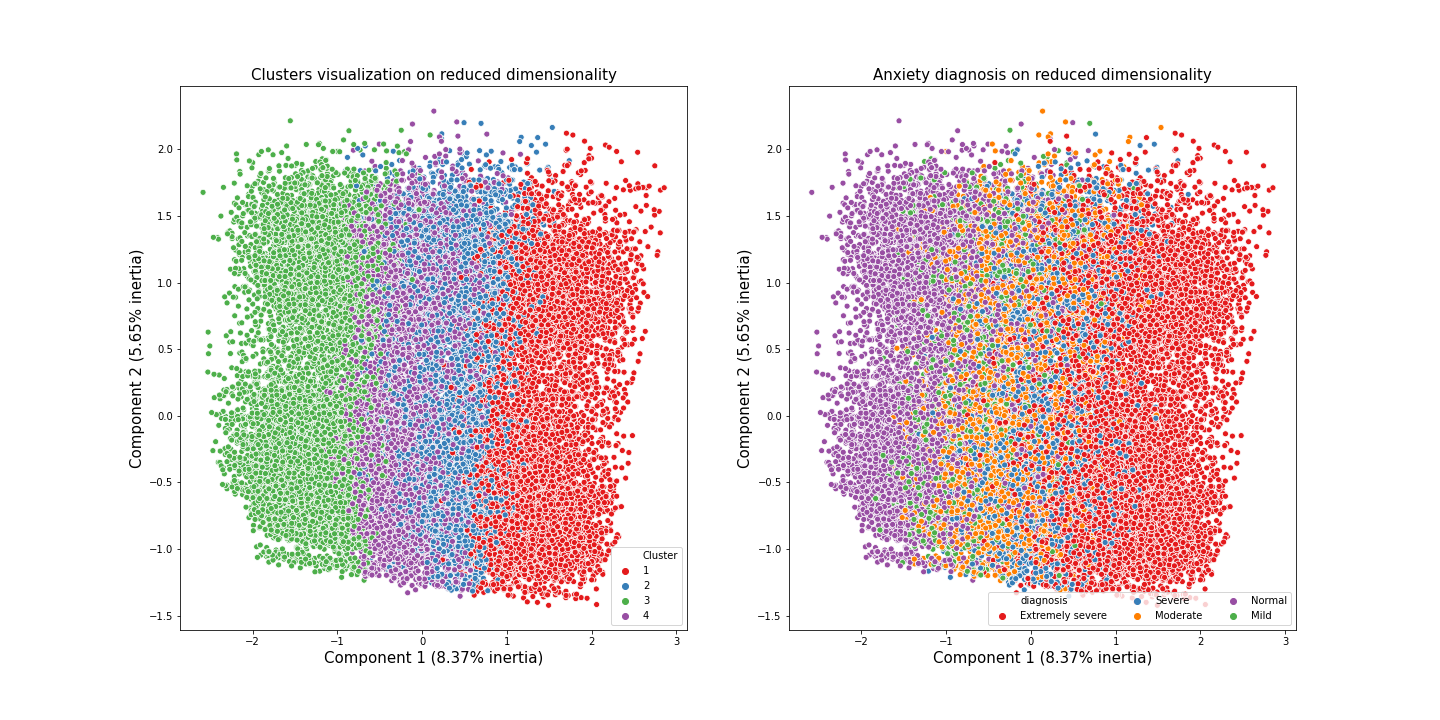
\includegraphics[width=\textwidth,height=\textheight,keepaspectratio]{Media/Pictures/anxiety_clusters.png} 
\label{clusters_ansiedad}
\end{figure}

En el cuadro \ref{matriz_depresion} se evidencia que así como para las condiciones anteriores, los clusters 1 y 3 tienen la mayor cantidad de casos con diagnósticos extremadamente severo y normal respectivamente. Lo particular para esta condición es que el cluster 2 presenta únicamente casos con diagnósticos extremadamente severo y severo con excepción de unos pocos casos con diagnostico moderado. Finalmente, el cluster 4 presenta en su mayoría casos con diagnostico moderado y un numero considerable de los demás diagnósticos con excepción de extremadamente severo. El cuadro  \ref{metricas_matriz_depresion} permite apreciar que las métricas para este modelo tienen valores similares a las condiciones anteriores pero son un poco menores.



\begin{table}[ht]
\centering
\caption{Matriz de confusión para depresión}
\begin{tabular}{lrrrr}
\toprule
Clusters &     1 &     2 &     3 &     4 \\
Depression\_Diagnosis &       &       &       &       \\
\midrule
Normal               &  0 &  0 &  7655 &  1198 \\
Mild                 &  13 &  0 &  1836 &  1937 \\
Moderate             &  209 &  7 &  1278 &  5583 \\
Severe               &  1218 &  2803 &  267 &  2188 \\
Extremely severe     &  7933 &  5619 &  15 &  0 \\
\bottomrule
\end{tabular}
\label{matriz_depresion} 
\end{table}%



\begin{table}[ht]
\centering
\caption{Métricas de los clusters de depresión}
\begin{tabular}{rr}
\toprule
 Van Dongen Criterion &  Adjusted Rand Score \\
\midrule
0.49 & 0.4 \\
\bottomrule
\end{tabular}
\label{metricas_matriz_depresion}
\end{table}%




La figura \ref{clusters_depresion} muestra que al igual que para las dos condiciones previas, el eje x coincide con la severidad de la condición. Al igual que para las previas condiciones, los diagnósticos leve, moderado y severo se superponen en el centro de la gráfica, estando particularmente presentes en el cluster 4 y en menor medida en el cluster 2. Así mismo, al igual que para la condición de ansiedad, se observa que la condición de extremadamente severo se encuentra dispersa hacia en centro del gráfico, lo cual se explica, al igual que para la condición de ansiedad, por una mayor presencia de casos con este diagnostico, estando de esta manera presente en los clusters 1 y 2.

\begin{figure}[hbt!]
\caption{Análisis de clusters para el diagnostico de depresión}
\centering
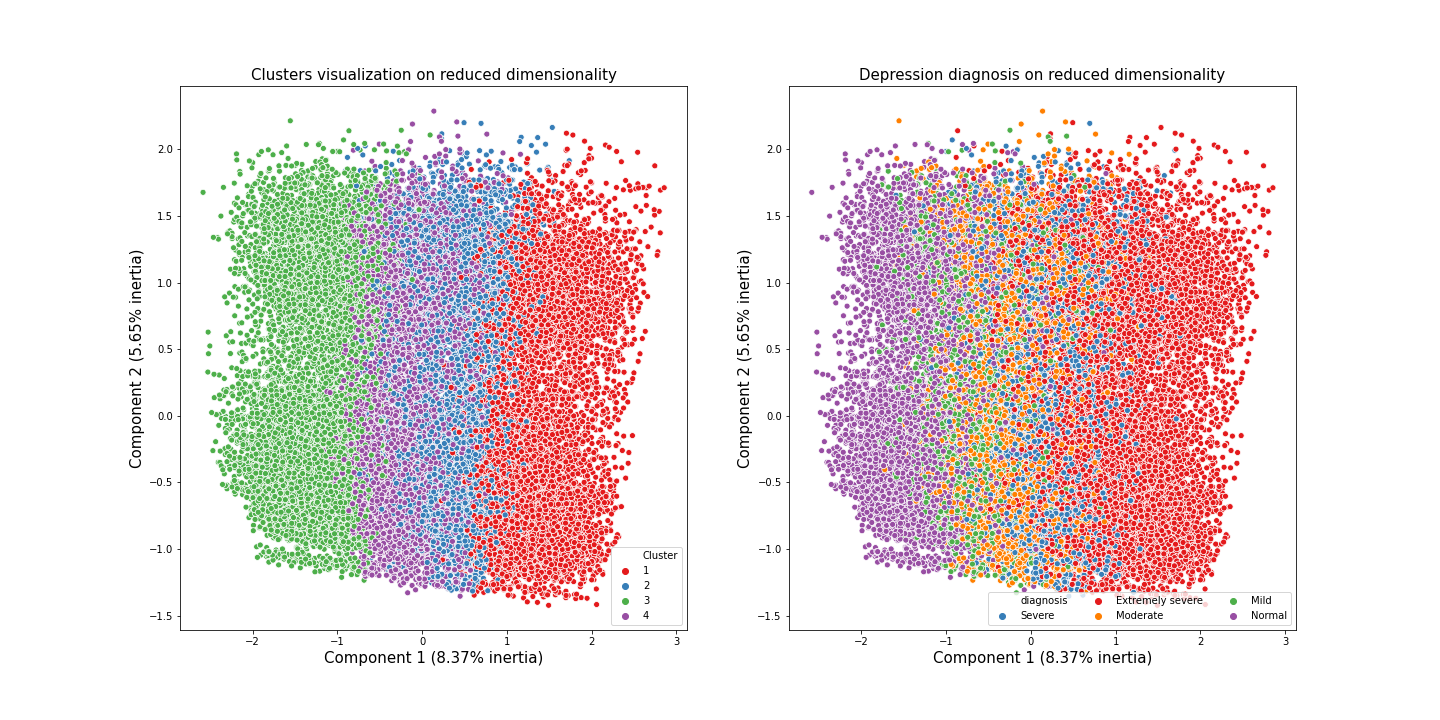
\includegraphics[width=\textwidth,height=\textheight,keepaspectratio]{Media/Pictures/depression_clusters.png} 
\label{clusters_depresion}
\end{figure}






